% !TeX spellcheck = cs_CZ
{\tikzset{external/prefix={tikz/CES/}}
 \tikzset{external/figure name/.add={ch06_}{}}
%---------------------------------------------------------------------------------------------------
% file CPP.tex
%---------------------------------------------------------------------------------------------------
\lstset{ %
  language=C++,                          % choose the language of the code
  basicstyle=\footnotesize\ttfamily,     % the size of the fonts that are used for the code
%  backgroundcolor=\color{gray},         % choose the background color. You must add 
                                         % \usepackage{color}
  commentstyle=\color{help}\textit,
  keywordstyle=\color{keyword}\textbf,
  breaklines=true,                       % sets automatic line breaking
  breakatwhitespace=true,                % sets if automatic breaks should only happen at whitespace
  showspaces=false,                      % show spaces adding particular underscores
  showstringspaces=true,                 % underline spaces within strings
  showtabs=true,                         % show tabs within strings adding particular underscores
  frame=none,	                           % adds a frame around the code - none, single
  tabsize=8,                             % sets default tabsize to 8 spaces
  captionpos=b,                          % sets the caption-position to bottom
  numbers=left,                          % where to put the line-numbers -none, left, right
  numberstyle=\footnotesize,             % the size of the fonts that are used for the line-numbers
  stepnumber=1,                          % the step between two line-numbers. If it's 1 each line
                                         % will be numbered
  xleftmargin=3em,                       % adjust left margin
}
%========================== Kapitola: Přehled jazyka C++============================================
\chapter{Programování v jazyku C++}
\minitoc

  \section{Úvodní slovo}
    \texttt{C++} je rozšířená verze jazyka \texttt{C}. \texttt{C++} zahrnuje vše, co je součástí 
    jazyka \texttt{C}, a přidává podporu objektově orientovaného programování (zkráceně 
    \texttt{OOP}). \texttt{C++} navíc obsahuje mnohá vylepšení, a prvky, které z něj jednoduše 
    dělají "lepší \texttt{C}", nezávisle na objektově orientovaném programování. Kromě několika 
    málo zanedbatelných výjimek platí, že \texttt{C} je podmnožinou jazyka \texttt{C++}.
  
    Poněvadž byl \texttt{C++} vytvořen pro podporu OOP, začne následující podkapitola popis\-em 
    \texttt{OOP}. Je důležité si uvědomit, že jazyka \texttt{C++} může byt použito i pro psaní 
    programů, které nejsou objektově orientovány. Tato kapitola, kromě představení nejdůležitějších 
    vlastností jazyka \texttt{C++}, diskutuje především o rozdílech mezi způsoby programování v 
    \texttt{C} a v \texttt{C++} \cite[p.~20]{Schildt}.
  
  \section{Objektově orientované programování}
    Objektově orientované programování je výkonný způsob jak přistupovat k úloze programování. Již 
    od raných začátků bylo programování spojováno s rozličnými metodologiemi. V každém kritickém 
    momentě během vývoje programování byly vytvářeny nové přístupy, které pomohly programátorům 
    zvládat stále složitější programy. První programy byly vytvářeny pouhým nastavením přepínačů na 
    panelu počítače. Tento postup byl vhodný pouze pro velmi malé programy. Později vytvořený jazyk 
    symbolických instrukcí již umožňoval psaní delších programů. K dalšímu vývoji došlo v roce 
    1955, kdy byl vytvořen první programovací jazyk vysoké úrovně - \texttt{FORTRAN}.
  
    S využitím programovacího jazyka vysoké úrovně byl programátor schopen psát programy o délce 
    několika tisících řádků. Nejstarší metodou použitou pro programování byl \emph{ad hoc} přístup 
    "všechno jde". Jestliže to bylo přípustné pro relativně krátké programy, pak u rozsáhlých 
    programů to vedlo k vytváření nečitelných a nezvládnutelných "špagety kódů"
  
    Eliminaci "špagety kódů" umožnil až vznik \emph{strukturovaných programovacích jazyků} v 
    šedesátých letech. Byly to jazyky \texttt{Algol} a \texttt{Pascal}. Volně lze interpretovat, že 
    je-li jazyk C strukturovaný, pak typ programování, které v něm provádíme, by se mohl označit 
    jako strukturované programování. Strukturované programování se opírá o dobře definované řídící 
    struktury, bloky kódů, vyloučení příkazů GOTO, lokální (stand-alone) podprogramy, které 
    podporují rekurzi, a lokální proměnné.
  
    Přestože strukturované programování přinášelo výborné výborné výsledky, když bylo použito pro 
    středně složité programy, v mnoha bodech zklamalo, když program přesáhl určitou velikost. K 
    tomuto účelu bylo vytvořeno objektově orientované programování. OOP vzalo nejlepší myšlenky 
    včleněné do strukturovaného programování a zkombinovalo je s výkonnými novými koncepty, které 
    dovolují organizovat programy mnohem efektivněji.
  
    Obecně všechny OOP jazyky sdílejí tři definované vlastnosti:
    \begin{itemize}\addtolength{\itemsep}{-0.5\baselineskip}
      \item zapouzdření (encapsulation),
      \item polymorfismus (polymorphism),
      \item dědičnost (inheritance).
    \end{itemize}
  
    \subsection{Třídy: první nahlédnutí}
      Snad nejdůležitějším samostatným prvkem jazyka C++ je \textbf{třída}. Je to mechanismus 
      používaný pro vytváření objektů. Jako taková, je třída srdcem mnoha prvků jazyka C++. Třídy 
      jsou pro programování v C++ tak významné, že je vhodné předložit na tomto místě jejich 
      stručný 
      přehled.
  
      \begin{definition}[Třída]
        \emph{Třída} je základním obecným pojmem klasifikace, jak při návrhu uspořádávat informace 
        do smysluplné entity. Základním pojmem je \emph{objekt}, \textbf{instance třídy}, jako 
        konkrétní případ realizace předpisu. Objekt si „pamatuje“ svůj stav (v podobě \textbf{dat} 
        čili \textbf{atributů}) a zveřejněním některých svých operací (nazývaných \textbf{metody}) 
        poskytuje rozhraní, jak s ním pracovat. Při používání objektu nás zajímá, jaké operace 
        (služby) poskytuje, ale ne, jakým způsobem to provádí - to je princip \emph{zapouzdření}. 
        Jestli to provádí sám nebo využije služeb jiných objektů, je celkem jedno. Vlastní 
        implementaci pak můžeme změnit (např. zefektivnit), aniž by se to dotklo všech, kteří 
        objekt používají.
  
        Abstrakce objektu, která v architektuře programu podchycuje na obecné úrovni podstatu všech 
        objektů podobného typu, se nazývá \textbf{třída}. Třída je předpis, jak vyrobit objekt 
        daného typu.
      \end{definition}
      
      \begin{example}
        Nechť má sousedka (chápejme ji jako objekt) má nějaké jméno, je nějak vysoká, umí chodit a 
        umí mluvit. Totéž platí i pro mne. Mohu tedy při modelování těchto dvou objektů, sousedky a 
        mě, abstrahovat od nepodstatných dílčích odlišností a díky této abstrakci vytvořit obecnou 
        třídu Člověk, která bude mít atributy jméno a příjmení (obojí je nějaký řetězec znaků) a 
        metody chodit a mluvit.
      \end{example}
  
      Třída je deklarována klíčovým slovem \lstinline[basicstyle=\ttfamily]!class!. Syntaxe 
      deklarace \lstinline[basicstyle=\ttfamily]!class! je podobná její struktuře. V obecné formě 
      vypadá takto
  
      %---------------------------------------------------------------
      \lstset{numbers=none}
      \begin{lstlisting}
      class jméno-třídy{
        // privatni-funkce a promenne
      public:
        // verejné funkce a promenne
      } seznam-objektů
      \end{lstlisting}
      %---------------------------------------------------------------
      Seznam objektů je v deklaraci třídy nepovinný. Stejně jako struktura, se  mohou  objekty 
      třídy deklarovat později. Zatímco jméno třídy je také nepovinné, z praktického hlediska je 
      vlastně vždy potřeba. Je to proto, že se jméno třídy stává novým typem jména použitého k 
      deklaraci objektů třídy.
  
      \textbf{Funkce a proměnné} deklarované uvnitř třídy jsou označeny jako \textit{členy této 
      třídy}. Znamená to, že jsou přístupné pouze pro ostatní členy třídy. Pro deklaraci členů 
      veřejné třídy se použije klíčové slovo \lstinline[basicstyle=\ttfamily]!public! s dvojtečkou. 
      Všechny funkce a proměn\-né deklarované za tímto specifikátorem jsou přístupné jak pro členy 
      třídy, tak i pro další části programu, které obsahují třídu.
  
      Toto je jednoduchá deklarace třídy:
  
      %---------------------------------------------------------------
      %\begin{lstlisting}[frame=trbl]{}
      \begin{lstlisting}{}
      class myclass{
        // privátní vzhledem k myclass
        int a;
      public:
        void set_a(int num);
        int get_a();
      };
      \end{lstlisting}
      %---------------------------------------------------------------
      Tato třída má pouze jednu privátní proměnnou nazvanou \lstinline[basicstyle=\ttfamily]!a! a 
      dvě veřejné funkce \lstinline[basicstyle=\ttfamily]!set_a()! a 
      \lstinline[basicstyle=\ttfamily]!get_a()!. Tyto funkce jsou deklarovány uvnitř třídy pomocí 
      jejich \textbf{prototypů}. Funkce, které jsou deklarovány jako součásti třídy se nazývají 
      \textit{členské funkce}.
  
      Jelikož je \lstinline[basicstyle=\ttfamily]!a! privátní, není dostupné pro žádný kód vně
      \lstinline[basicstyle=\ttfamily]!myclass!. Ovšem funkce 
      \lstinline[basicstyle=\ttfamily]!set_a()! a
      \lstinline[basicstyle=\ttfamily]!get_a()! jsou členy 
      \lstinline[basicstyle=\ttfamily]!myclass!, takže 
      mají k \lstinline[basicstyle=\ttfamily]!a! přístup. \lstinline[basicstyle=\ttfamily]!set_a()! 
      a
      \lstinline[basicstyle=\ttfamily]!get_a()! jsou deklarovány jako veřejné členy 
      \lstinline[basicstyle=\ttfamily]!myclass! a mohou být volány každou částí programu, která 
      \lstinline[basicstyle=\ttfamily]!myclass! obsahuje.
  
      Ačkoliv jsou funkce \lstinline[basicstyle=\ttfamily]!set_a()! a 
      \lstinline[basicstyle=\ttfamily]!get_a()!  deklarovány v 
      \lstinline[basicstyle=\ttfamily]!myclass!, nejsou ještě definovány. Aby jsem definoval 
      členskou funkci, musím spojit typové jméno třídy se jménem funkce. To se udělá uvozením jména 
      funkce jménem třídy se dvojicí dvojteček. Dvojice dvojteček se nazývá \textit{operátor 
      rozlišení oblasti} (scope resolution operator). Následující příklad ukazuje, jak jsou členské 
      funkce \lstinline[basicstyle=\ttfamily]!set_a()! a    
      \lstinline[basicstyle=\ttfamily]!get_a()! definovány:
      %---------------------------------------------------------------
      \begin{lstlisting}{}
      void myclass::set_a(int num)
      {
        a = num;
      }
  
      int myclass::get_a()
      {
       return a;
      }
      \end{lstlisting}
      %---------------------------------------------------------------
      Jak \lstinline[basicstyle=\ttfamily]!get_a()!, tak i 
      \lstinline[basicstyle=\ttfamily]!set_a()! 
      mají přístup k \lstinline[basicstyle=\ttfamily]!a!, které je privátní v 
      \lstinline[basicstyle=\ttfamily]!myclass!. Poněvadž
      \lstinline[basicstyle=\ttfamily]!get_a()! i \lstinline[basicstyle=\ttfamily]!set_a()! jsou 
      členy \lstinline[basicstyle=\ttfamily]!myclass!, mohou přímo přistupovat k jejím soukromým 
      datům.
  
      Obecně se pro definici členské funkce musí použít následující tvar:
      %---------------------------------------------------------------
      \begin{lstlisting}{}
      re-type jméno-třídy::jmeno-funkce(seznam-parametru)
      {
      // telo funkce
      }
      \end{lstlisting}
      %---------------------------------------------------------------
      Deklarace \lstinline[basicstyle=\ttfamily]!myclass! nedefinuje žádný objekt typu 
      \lstinline[basicstyle=\ttfamily]!myclass!. Definuje pouze typ objektu, který bude vytvořen, 
      když bude deklarován. Pro vytvoření objektu se použije jako specifikátor jméno třídy. 
      Například tento řádek deklaruje dva objekty typu \lstinline[basicstyle=\ttfamily]!myclass!:
      %---------------------------------------------------------------
      \begin{lstlisting}{}
        myclass ob1, ob2; //toto jsou objekty typu myclass
      \end{lstlisting}
      %---------------------------------------------------------------
      Jakmile je vytvořen objekt třídy, může se program odkazovat na jeho veřejné členy pomocí 
      tečkových operátorů bezmála takovým způsobem, jímž jsou prvky struktury zpřístupněny. Dle 
      předcházející deklarace objektů volají následující příkazy 
      \lstinline[basicstyle=\ttfamily]!set_a()! pro objekty 
      \lstinline[basicstyle=\ttfamily]!ob1! a \lstinline[basicstyle=\ttfamily]!ob2!:
      %---------------------------------------------------------------
      \begin{lstlisting}{}
        ob1.set_a(10); // nastaví verzi ob1 na 10
        ob2.set_a(99); // nastaví verzi ob2 na 99
      \end{lstlisting}
      %---------------------------------------------------------------
      Každý objekt obsahuje vlastní kopii všech dat deklarovaných uvnitř třídy. Znamená to, že 
      \lstinline[basicstyle=\ttfamily]!a! náležející \lstinline[basicstyle=\ttfamily]!ob1! je 
      odlišné a různé od \lstinline[basicstyle=\ttfamily]!a! navázaného na 
      \lstinline[basicstyle=\ttfamily]!ob2!.
  
      \begin{example}
         Tento program předvádí \lstinline[basicstyle=\ttfamily]!myclass!, popsanou výše v textu. 
         Nastavuje hodnoty \lstinline[basicstyle=\ttfamily]!a! pro 
         \lstinline[basicstyle=\ttfamily]!ob1! a 
         \lstinline[basicstyle=\ttfamily]!ob2!, a pak zobrazuje hodnotu a pro každý objekt.
         % \marginpar{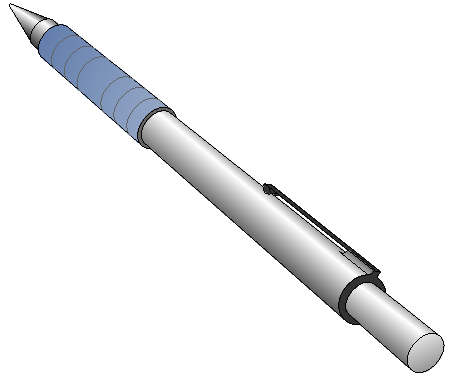
\includegraphics[width=0.05\textwidth]{pen.pdf}}       
         %---------------------------------------------------------------
         \lstinputlisting{../src/CES/CPP/HS_37_myclass.cpp}
         %---------------------------------------------------------------
         Program by měl na obrazovce zobrazit hodnoty \lstinline[basicstyle=\ttfamily]!10! a 
         \lstinline[basicstyle=\ttfamily]!99!.
      \end{example}
  
      \begin{example}
        V \lstinline[basicstyle=\ttfamily]!myclass! z předchozího příkladu je 
        \lstinline[basicstyle=\ttfamily]!a! privátní. Znamená to, že k ní mohou přímo přistupovat 
        pouze členské funkce z \lstinline[basicstyle=\ttfamily]!myclass!. (To je důvodem, proč je 
        vyžadována veřejná funkce \lstinline[basicstyle=\ttfamily]!get_a()!). Tedy při pokusu o 
        přístup k privátnímu členu třídy z některé části programu, která není členem třídy, objeví 
        s při překladu chyba. Pokud je \lstinline[basicstyle=\ttfamily]!myclass! definována tak, 
        jak bylo předvedeno v předešlém příkladě, pak následující volání funkce 
        \lstinline[basicstyle=\ttfamily]!main()! zapříčiní chybu:
  
        %---------------------------------------------------------------
        \begin{lstlisting}
        // Toto je fragment obsahující chybu.
        #include<iostream>
        using namespace std;
        int main()
        {
          myclass ob1, ob2;
          ob1.a = 10; // ERROR! nemůže přistupovat
                      // k privátnímu členu
          ob2.a = 99; // dle nečlenských funkcí.
  
          cout << ob1.get_a() << "\n";
          cout << ob2.get_a() << "\n";
  
          return 0;
        }
       \end{lstlisting}
       %---------------------------------------------------------------
      \end{example}
  
      \begin{example}
        Stejně jako mohou existovat funkce veřejného členu, mohou existovat i proměnné veřejného 
        členu. Jestliže například \lstinline[basicstyle=\ttfamily]!a! bylo deklarováno ve veřejné 
        části \lstinline[basicstyle=\ttfamily]!myclass!, lze se na ně odkazovat z kterékoliv části 
        programu, jak je předvedeno dále:
        % \marginpar{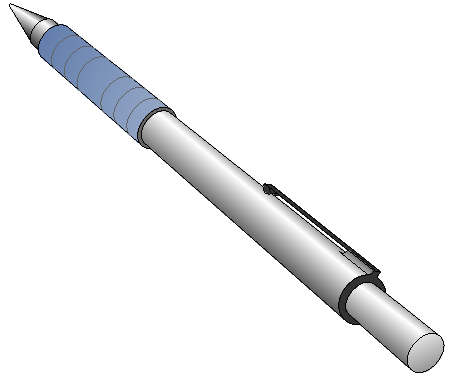
\includegraphics[width=0.09\textwidth]{pen.pdf}}
        %---------------------------------------------------------------
          \begin{lstlisting}
          #include<iostream>
          using namespace std;
  
          class myclass{
          public:
          // nyní je a veřejné
          int a;
          // a  nyní není potřeba set_a() a get_a()
          };
  
          int main()
          {
          myclass ob1, ob2;
  
          ob1.a = 10;
          ob2.a = 99;
  
          cout << ob1.a << "\n";
          cout << ob2.a << "\n";
  
          return 0;
          }
          \end{lstlisting}
        %---------------------------------------------------------------
        Protože je v tomto příkladě \lstinline[basicstyle=\ttfamily]!a! deklarováno jako veřejný 
        člen \lstinline[basicstyle=\ttfamily]!myclass!, je přímo přístupné z 
        \lstinline[basicstyle=\ttfamily]!main()!. Pro přístup k \lstinline[basicstyle=\ttfamily]!a! 
        je použit tečkový operátor. Obvykle, když se volá členská funkce nebo se přistupuje k 
        členské proměnné z vnějšího prostředí mimo třídu, je nutná plná specifikace daná jménem 
        objektu i s tečkovým operátorem následovaným jménem člena, aby bylo jasné, na kterého člena 
        objektu se odkazuje.
      \end{example}
  
      \begin{example}\label{stack1}
        Aby byla ukázána síla objektů, následující program vytváří třídu pojmenovanou 
        \lstinline[basicstyle=\ttfamily]!stack!, která implementuje zásobník použitelný například 
        pro uchování znaků:
        %---------------------------------------------------------------
        \lstinputlisting{../src/CES/CPP/HS_39_stack.cpp}
        %---------------------------------------------------------------
        Program zobrazí následující výstupy:
        \begin{center}
        Pop s1: c\linebreak
        Pop s1: b\linebreak
        Pop s1: a\linebreak
        Pop s2: z\linebreak
        Pop s2: y\linebreak
        Pop s2: x
        \end{center}
  
        Podívej se na program ještě jednou. Třída \lstinline[basicstyle=\ttfamily]!stack! obsahuje 
        dvě privátní proměnné: \lstinline[basicstyle=\ttfamily]!stck! a 
        \lstinline[basicstyle=\ttfamily]!tos!. Pole 
        \lstinline[basicstyle=\ttfamily]!stck! uchovává znaky umístěné v zásobníku a 
        \lstinline[basicstyle=\ttfamily]!tos! obsahuje index horní úrovně zásobníku. Veřejné funkce 
        zásobníku jsou \lstinline[basicstyle=\ttfamily]!init()!, 
        \lstinline[basicstyle=\ttfamily]!push()! a
        \lstinline[basicstyle=\ttfamily]!pop()! a slouží k inicializaci zásobníku, vkládání hodnoty 
        a k vyjmutí hodnoty. Uvnitř \lstinline[basicstyle=\ttfamily]!main()! jsou vytvořeny dva 
        zásobníky \lstinline[basicstyle=\ttfamily]!s1! a \lstinline[basicstyle=\ttfamily]!s2! a do 
        každého z nich jsou vloženy tři znaky. Je důležité uvědomit si, že každý zásobníkový objekt 
        je oddělený od druhého. To znamená, že znaky vložené do         
        \lstinline[basicstyle=\ttfamily]!s1! nemohou žádným způsobem ovlivnit znaky vložené do 
        \lstinline[basicstyle=\ttfamily]!s2!. Každý objekt obsahuje vlastní kopii 
        \lstinline[basicstyle=\ttfamily]!stck! a \lstinline[basicstyle=\ttfamily]!tos!. To je 
        základní princip pro pochopení objektů. Ačkoliv všechny objekty třídy sdílejí své členské 
        funkce, každý objekt vytváří a udržuje svá vlastní 
        data.
      \end{example}	
  
    \subsection{Některé rozdíly mezi C a C++}
      Ačkoliv je jazyk C++ rozšířenou množinou jazyka C, existují mezi nimi drobné rozdíly a bylo 
      by dobré se s nimi na začátku seznámit. Především, když v C nemá funkce žádné parametry, její 
      protyp má v seznamu parametrů funkce slovo \lstinline[basicstyle=\ttfamily]!void!. Například 
      když v "céčku" funkce nazvaná \lstinline[basicstyle=\ttfamily]!fl()! nemá parametry (a vrací 
      \lstinline[basicstyle=\ttfamily]!char!), pak její prototyp bude vypadat následovně:
      %---------------------------------------------------------------
      \begin{lstlisting}
      char fl(void);
      \end{lstlisting}
      %---------------------------------------------------------------
      Přestože v C++ zůstává void stále jako volitelný, bude se prototyp pro 
      \lstinline[basicstyle=\ttfamily]!fl()! psát běžně takto:
      %---------------------------------------------------------------
      \begin{lstlisting}
      char fl();
      \end{lstlisting}
      %---------------------------------------------------------------
  
      C++ se odlišuje od C tím, že je v něm specifikován prázdný seznam parametrů. Kdyby se 
      předchozí prototyp objevil v programu C, pak se to bude chápat, že o parametrech nebylo 
      řečeno nic. V C++ to znamená, že funkce nemá parametry. Proto tedy v předchozím příkladě 
      nebyl využit k deklaraci prázdného seznamu explicitně parametr void. (Použití parametru void 
      k deklaraci prázdného  seznamu parametrů není zakázáno; je to pouze nadbytečné. Jelikož 
      většina programů C++ usiluje o téměř posvátným zanícením o výkonnost,neuvidíš téměř nikdy, že 
      by bylo void tímto způsobem použito.) Zapamatuj si, že v C++ jsou následující dvě deklarace 
      zcela rovnocenné:
      %---------------------------------------------------------------
      \begin{lstlisting}
      char fl();
      char fl(void);
      \end{lstlisting}
      %---------------------------------------------------------------
  
      Další drobná diference mezi C a C++ spočívá v tom, že v programech C++ musí mít všechny 
      funkce prototypy. Zapamatuj si, že v C jsou prototypy doporučeny, ale technicky jsou 
      nepovinné. V C++ jsou však vyžadovány. Jak je patrno z příkladu v předchozí části, prototyp 
      členské funkce obsažený v třídě slouží rovněž jako její obecný prototyp a žádný další 
      samostatný prototyp již není požadován. Třetím rozdílem mezi C a C++ je, když je funkce 
      deklarována aby vracela hodnotu, musí hodnotu opravdu vracet. Jestliže má totiž funkce jiný 
      návratový typ než void, musí pak každý příkaz return uvnitř funkce obsahovat hodnotu. V C 
      není vyžadováno, aby vracely hodnotu funkce, které nejsou void. Jestliže hodnota neexistuje, 
      "vrací se" jakási nahodilá hodnota.
   
      Jestliže v C nespecifikujete explicitně návratový typ funkce, předpokládá se návratový typ 
      integer. V C++ bylo toto pravidlo potlačeno, a proto musíš explicitně deklarovat všechny 
      návratové typy funkcí. Další rozdíl mezi C a C++ je, že v programech C budeš muset brát ohled 
      na to, kde mohou být lokální proměnné deklarovány. V C mohou být lokální proměnné deklarovány 
      pouze na začátku bloku před všemi "výkonnými" příkazy. V C++ mohou být lokální proměnné 
      deklarovány kdekoliv. Výhodou tohoto přístupu je, že lokální proměnné mohou být deklarovány 
      ta, kde budou poprvé použity, což může napomoci v prevenci před nechtěnými vedlejšími účinky.
  
      Konečně také v C++ definuje datový typ \lstinline[basicstyle=\ttfamily]!bool! pro uložení  
      hodnot \lstinline[basicstyle=\ttfamily]!Boolean! (popř. pravda/nepravda). C++ rovněž definuje 
      klíčová slova \lstinline[basicstyle=\ttfamily]!true! a   
      \lstinline[basicstyle=\ttfamily]!false!, 
      která jsou jedinými hodnotami, které může hodnota typu 
      \lstinline[basicstyle=\ttfamily]!Boolean! nabývat. V C++ je výstupní hodnotou relačních a 
      logických operátorů hodnota typu \lstinline[basicstyle=\ttfamily]!bool! a všechny 
      podmíněné příkazy musí hodnotu bool vyhodnocovat. V C je hodnota 
      \lstinline[basicstyle=\ttfamily]!true! nenulová a hodnota 
      \lstinline[basicstyle=\ttfamily]!false! odpovídá nule. Tak je to i v C++, poněvadž při 
      použití v booleánských výrazech je každá nenulová hodnota automaticky převedena na    
      \lstinline[basicstyle=\ttfamily]!true! a každá nulová hodnota je převedena na 
      \lstinline[basicstyle=\ttfamily]!false!. Funguje to i opačným směrem. Když je booleánská 
      hodnota použita ve výrazech \lstinline[basicstyle=\ttfamily]!integer!, pak se 
      \lstinline[basicstyle=\ttfamily]!true! převádí na \lstinline[basicstyle=\ttfamily]!1! a 
      \lstinline[basicstyle=\ttfamily]!false! na \lstinline[basicstyle=\ttfamily]!0!. Přidání 
      \lstinline[basicstyle=\ttfamily]!bool! umožňuje důkladnější ověřování typů a poskytuje 
      způsob, jak navzájem rozlišovat \lstinline[basicstyle=\ttfamily]!Boolean! a     
      \lstinline[basicstyle=\ttfamily]!integer!. Využívání je samozřejmě nepovinné, ale
      \lstinline[basicstyle=\ttfamily]!bool! je nejpohodlnější.
  
    \subsection{Úvod do přetěžování funkcí}
      Po třídách je snad nejdůležitější a vše postupující vlastností C++ přetě\-žování funkcí. 
      Přetěžování funkcí nejen poskytuje mechanismus jímž C++ poskytuje jeden typ polymorfismu, ale 
      také utváří základ, na němž může být programovací prostředí dynamicky rozšiřováno. Kvůli 
      důležitosti přetěžování je v následujících odstavcích předložen stručný úvod. \footnote{V C++ 
      lze přetěžovat i operátory.}
  
      V C++ mohou dvě nebo více funkcí sdílet stejné jméno, pokud se liší typy jejich argumentů 
      nebo jejich počet anebo se liší obojí.
  
      Je velmi snadné přetížit funkci: jednoduše deklaruješ a definuješ všechny požadované verze. 
      Správnou verzi překladač automaticky vybere dle počtu nebo typu argumentů použitých při 
      volání funkce.
  
      \begin{example}
        Následující program definuje tři funkce pro výpočet absolutní hodnoty nazvané 
        \lstinline[basicstyle=\ttfamily]!abs()! - pro každý typ dat jednu.
        %---------------------------------------------------------------
        \lstinputlisting{../src/CES/CPP/HS_46_abs.cpp}
        %---------------------------------------------------------------
        \end{example}
  
        Překladač automaticky volá správně jednu ze tří verzí 
        \lstinline[basicstyle=\ttfamily]!abs()! dle typu dat, která jsou uvedena v argumentu. 
        Program vytvoří následující výstup:
        \begin{center}
          In integer abs()
          Absolute value of -10: 10
    
          In long abs()
          Absolute value of -10L: 10
    
          In double abs()
          Absolute value of -10.01: 10.01
        \end{center}
  
        Uvedený příklad je velmi jednoduchý, nicméně ukazuje význam přetěžování funkcí. Jelikož lze 
        jediné jméno použít k popisu obecné třídy činností, je umělá složitost, která vyplývá z 
        použití tří mírně odlišných jmen - v tomto případě \lstinline[basicstyle=\ttfamily]!abs()!, 
        \lstinline[basicstyle=\ttfamily]!labs()! a \lstinline[basicstyle=\ttfamily]!fabs()! - 
        snadno eliminována.
  
        \begin{example}\label{date}
        %---------------------------------------------------------------
        \lstinputlisting{../src/CES/CPP/HS_47_date.cpp}
        %---------------------------------------------------------------
        \end{example}
  
      Příklad \ref{date} ilustruje jak může přetížení funkce zajistit mnohem při\-rozenější přístup 
      k funkci. Protože je poměrně běžné, že je datum reprezentováno buď řetězcem, nebo třemi 
      celočíselnými hodnotami obsahující den, měsíc a rok, záleží jen na uživateli, aby vybral tu 
      nejpohodlnější formu, dle dané situace
  
    \subsection{Práce s ukazateli}  
  
      \begin{example} Práce s ukazateli:\label{CPP:ex_pointer1}
      %---------------------------------------------------------------
      \lstinputlisting{../src/CES/CPP/GP_548_point.cpp}
      %---------------------------------------------------------------
      Výstup programu:
        \begin{verbatim}
          num is 123
          The address of num is 0x28ff44
          *p_num is 123
          p_num is 0x28ff44
          \end{verbatim}
      \end{example}
      
      \begin{example}\label{CPP:ex_swap} Napište funkci \texttt{swap} která prohodí hodnoty dvou 
      proměnných typu \texttt{int}. Výsledek funkce \texttt{swap} vytiskněte na výstupu terminálu.
      %---------------------------------------------------------------
      \lstinputlisting{../src/CES/CPP/GP_551_swap.cpp}
      %---------------------------------------------------------------
      Výstup programu:
        \begin{verbatim}
        Before swap, i is 10 and j is 20
        
        After swap, i is 20 and j is 10
        \end{verbatim}
      \end{example}
      
      \begin{example}\label{CPP:ex_scitej_nasob} Následující příklad ukazuje použití 
      \textbf{ukazatele na funkci}. Program se nejprve zeptá, zda se má provádět sčítání nebo 
      násobení. Podle této odpovědi vloží do proměnné \texttt{operation} ukazatel na funkci 
      \texttt{add} nebo na funkci \texttt{multiply}. Dále zadáme dvě čísla, která se použijí jako 
      parametry vybrané funkce.
      %---------------------------------------------------------------
      \lstinputlisting{../src/CES/CPP/WEB_01_pointer_to_func.cpp}
      %---------------------------------------------------------------
      \end{example}             
  
  %============ Kapitola: Úvod do tříd =============================================================
  \section{Úvod do tříd}
  
    \subsection{Funkce konstruktor a destruktor}
      Je zcela běžné, že některé části programu vyžadují inicializaci. Potřeba inicializace je 
      mnohem častější, když se pracuje s objekty. K ošetření této situace poskytuje C++ funkci 
      konstruktor, která může být vložena do deklarace třídy. Všechny inicializace, které je nutno 
      na objektu provést, může automaticky vykonat konstruktor. Konstruktor má stejné jméno jako 
      třída, jejíž je součástí a nemá návratový typ (není to ani povoleno). Následující příklad 
      ukazuje krátkou třídu, jež obsahuje konstruktor.
  
      %---------------------------------------------------------------
      \lstinputlisting{../src/CES/CPP/HS_55_myclass.cpp}
      %---------------------------------------------------------------
  
      V tomto jednoduchém příkladě je hodnota \lstinline[basicstyle=\ttfamily]!a! inicializována 
      konstruktorem \lstinline[basicstyle=\ttfamily]!myclass()!. Konstruktor je volán při vytváření 
      objektu \lstinline[basicstyle=\ttfamily]!ob!. Objekt je vytvářen tehdy, když se provádí jeho 
      deklarační příkaz. V C++ je deklarační příkaz proměnné vlastně "příkazem činnosti". Když se 
      programuje v C, lze deklarační příkazy považovat za zavádění proměnných. Ovšem v C++, 
      poněvadž objekt může mít konstruktor, bude ve skutečnosti příkaz pro deklaraci proměnné 
      vyvolávat celou řadu činností.
  
      Pro globální objekty je konstruktor objektu volán jen jednou, když se program začíná poprvé 
      spouštět. Pro lokální objekty je konstruktor volán pokaždé, když je prováděn deklarační 
      příkaz. Doplňkem konstruktoru je destruktor. Tato funkce volána, když je objekt rušen. Když 
      se pracuje s objekty, je běžné, že se musí provést v souvislosti s rušením objektu určité 
      akce (např. uvolnění zabrané paměti). Následující třída již destruktor obsahuje:
      %---------------------------------------------------------------
      \lstinputlisting{../src/CES/CPP/HS_56_myclass.cpp}
      %---------------------------------------------------------------
  
      Destruktor třídy je volán, když je objekt rušen. Lokální objekty jsou rušeny, když odcházejí 
      mimo oblast. Globální objekty jsou rušeny, když program končí.
  
      Není možné získat adresu konstruktoru nebo destruktoru.
      \begin{example}
        Třída \lstinline[basicstyle=\ttfamily]!stack! vytvořená v příkladu \ref{stack1} vyžadovala 
        inicializační funkci k nastavení proměnné pro index zásobníku. To je přesně ten druh 
        operací, pro něž byl konstruktor navržen. Zde je vylepšení verze třídy 
        \lstinline[basicstyle=\ttfamily]!stack!, která používá konstruktor pro automatickou 
        inicializaci zásobníkového objektu po jeho vytvoření:
        %---------------------------------------------------------------
        \lstinputlisting{../src/CES/CPP/HS_57_stack.cpp}
        %---------------------------------------------------------------
        Je Vidět, že úloha inicializace je konstruktorem provedena automaticky lépe, než pomocí 
        samostatné funkce, která by musela být explicitně volána programem. Když je inicializace 
        provedena automaticky při vytváření objektu, eliminuje to možnost, že by kvůli výskytu 
        chyby inicializace neproběhla. Je to další cesta, jak omezit složitost programu.
      \end{example}
      \begin{example}
        Tento příklad předvádí nutnost existence nejen konstruktoru, ale i destruktoru. Vytváří se 
        zde jednoduchá řetězcová třída, nazvaná \lstinline[basicstyle=\ttfamily]!strtype!, která 
        obsahuje řetězec a jeho délku. Když je objekt \lstinline[basicstyle=\ttfamily]!strtype! 
        vytvořen, je mu přidělena paměť pro uložení řetězce a jeho počáteční hodnota je nastavena 
        na \lstinline[basicstyle=\ttfamily]!0!. Když je objekt     
        \lstinline[basicstyle=\ttfamily]!strtype! zrušen, je paměť uvolněna.
        %---------------------------------------------------------------
        \lstinputlisting{../src/CES/CPP/HS_59_string.cpp}
        %---------------------------------------------------------------
      \end{example}
      Tento program používá pro přidělení a uvolnění paměti funkce 
      \lstinline[basicstyle=\ttfamily]!malloc! a \lstinline[basicstyle=\ttfamily]!free! Přestože to 
      funguje perfektně, dále je ukázáno, že v C++ se používá jiný způsob pro dynamickou správu 
      paměti.   

} % tikzset
%---------------------------------------------------------------------------------------------------
\printbibliography[title={Seznam literatury}, heading=subbibliography]
\addcontentsline{toc}{section}{Seznam literatury}